\documentclass{article}

\usepackage[utf8]{inputenc}
\usepackage{braket}
\usepackage{enumitem}
\usepackage{multirow}
\usepackage{xcolor}
\usepackage[T1]{fontenc}
% \usepackage[french]{babel}
\usepackage{amssymb}
\usepackage{mathtools}
\usepackage{ntheorem}
\usepackage{amsmath}
\usepackage{amssymb}
\usepackage[ a4paper, hmargin={2cm, 2cm}, vmargin={2cm, 2cm}]{geometry}
\usepackage{hyperref}
\usepackage{capt-of}

\usepackage{tikz}
\usetikzlibrary{angles,quotes}

\theoremstyle{plain}
\theorembodyfont{\normalfont}
\theoremseparator{~--}
\newtheorem*{define}{Definition}%[section]
\newtheorem*{ex}{Example}%[section]
\newtheorem*{obs}{Observation}%[section]

\newcommand{\norm}[1]{\left\lVert#1\right\rVert}

\usepackage{hyperref}
\hypersetup{
    colorlinks,
    citecolor=black,
    filecolor=black,
    linkcolor=blue,
    urlcolor=blue
}

\title{TD n$^\circ$2}
\author{Valeran MAYTIE}
\date{}

\begin{document}
  \maketitle
  
  An object $A$ in category $\mathcal C$ is called \underline{terminal} when
  there exists exactly one morphism $C \to A$ for any object $C$ of $\mathcal C$

  \begin{enumerate}
    \item What is a terminal object in an ordered set seen as an ordered
      category.
    \item Describe a terminal object of {\bf Set} and{\bf Top} and Graph, the
      category graph and graph homomorphism.
    \item Show that if $A$ is terminal and $f : A \to B$ is an isomorphism then B
      is terminal too.
    \item Suppose that $A$ and $B$ are terminal object in $\mathcal C$ show that
      exists an isomorphism $A \xrightarrow{f} B$ is unique.
  \end{enumerate}

  \underline{\bf Correction} :

  \begin{enumerate}
    \item A terminal object in an ordered set is \underline{the} maximum.
    \item Any singleton in {\bf Set} or in {\bf Top} and the graph for the
      category graph.
    \item Let $C \in \mathcal C$ and $g$ the unique morphism from $C$ to $A$.
      Then $f \circ g$ is a morphism from $C$ to $B$. \\ Let $h \in Hom(C, B)$,
      then $f \circ h \in Hom(C, A) = \{g\}$. So we have $h = f \circ g$.

      \begin{center}
      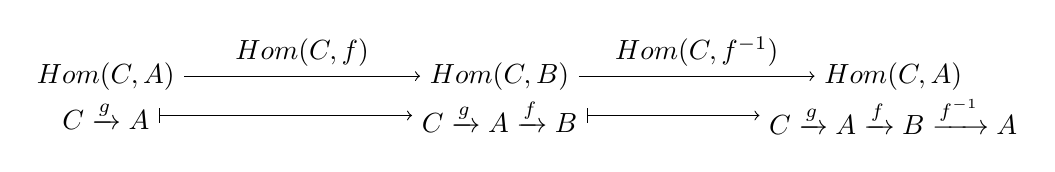
\begin{tikzpicture}
        \node (CA) at (-5, 0) {$Hom(C, A)$};
        \node (F0) at (-5, -0.5) {$C \xrightarrow{g} A$};

        \node (CB) at ( 0, 0) {$Hom(C, B)$};
        \node (F1)  at ( 0, -0.5) {$C \xrightarrow{g} A \xrightarrow{f} B$};

        \node (CA') at ( 5, 0) {$Hom(C, A)$};
        \node (F2)  at ( 5, -0.5) {$C \xrightarrow{g} A \xrightarrow{f} B
          \xrightarrow{f^{-1}} A$};

        \draw[->] (CA) to node[above] {$Hom(C, f)$} (CB);
        \draw[->] (CB) to node[above] {$Hom(C, f^{-1})$} (CA');
        \draw[|->] (F0) to (F1);
        \draw[|->] (F1) to (F2);

      \end{tikzpicture}
      \end{center}

    \item Let $f : A \to B$ and $g : B \to A$ (unique). We have $g \circ f : A \to A =
      Id_A$ (A is terminal) and $f \circ g : B \to B$ (B is terminal). We show
      that $g$ is the inverse of $f$ so $f$ is an isomorphism and it is unique. 
  \end{enumerate}

\end{document}
